


\clearpage
\setcounter{page}{1}


% \maketitlesupplementary %This messes up figure placement


\section{User Interface}

As a followup to \cref{sub:image_selection_process}, we discuss a specialized user interface we have developed for the manual annotation of this dataset, dramatically reducing the effort, time and cost of doing so.

Manual annotation, though less expensive than manual image matting (costing around \$30,000 and a few months), remains costly and time-consuming. To streamline this process, we've developed web-based program specifically for the task of selecting the best matte for subjects.

Along with the dataset, this tool will also be released to the public domain - in order to help people view and interact with this dataset before downloading it, as well as allowing people to easily expand it later on.

This tool simplifies the task by enabling annotators to quickly choose the best image from a set by simply clicking on it \cref{fig:ui}. Because it is web-based, it allows easy distribution of the annotation task: instead of having workers download the images to their local machines, terabytes of data can be streamed as they need it. Some key UI features include easy background color switching, alpha mask viewing with a single key-press, and workload distribution among multiple workers for parallel processing. 

Annotators are required to work with a dataset comprising RGBA images, which poses a challenge since there are no RGBA monitors — all physical pixels on a screen possess only RGB values. To circumvent this, we enable users to quickly view the alpha channel for samples and alternate the background color. This approach provides a clearer understanding of how the alpha mask influences the images.


% When the user's mouse is hovered over an image and the space bar is pressed, it zooms to full-screen. And when the letter `a' is pressed, it shows the alpha mask for that sample. This is better than zooming in manually to each sample, saving time and thus reducing the cost of annotation. There are many such quality of life features included like this.

This UI also includes search functionality as well, letting users search for images based on their captions. In \cref{fig:ui}, you can see that in the caption ``A crystal clear icicle hanging from a frozen branch'', the word ``icicle'' is bold and glowing - indicating the search term that matches that caption. There, the search term was ``icicle''. And in \cref{fig:tagging}, the search term ``letter'' was used.

Users can also tag images with tags such as ``\#nsfw,'' ``bad,'' and several other optional custom tags. Tags have many use cases, including: 
\begin{enumerate}
    \item It allows for the explicit annotation of poorly generated samples that lack good matting. Although this is a rare case, it still needs to be addressed.
    \item It enables the categorization of samples. For instance, the ``\#nsfw'' tag, represented as a button below the image samples, when activated for a given sample, marks that sample as not safe for work.
    \item It permits marking samples as ``\#idk'', which indicates that the sample requires review by another annotator. Since tags are searchable, if the user searches ``\#idk'', all samples marked as such will appear and can be reviewed.
\end{enumerate}


A live server for our dataset, along with the code and a user manual will be released for free to the public along with this paper. We hope by doing so we can encourage others to help grow the manually annotated portion of this dataset further.




\section{Additional Dataset Statistics}
Our data-set contains both safe-for-work and NSFW content, which is labeled as such. Approximately $.15\%$ of the samples in our dataset are flagged NSFW, as determined by a combination of the human annotators and a check for over 3000 blacklisted keywords present in the subjects. 

Additionally, the dataset contains a mix of shadows and non-shadows - as some samples will include soft shadows in their alpha-matte. 

The whole dataset generation process was accomplished on 32 A100 GPUs over the span of three weeks, plus an additional two months of human annotation with a budget of \$30000 USD. 

As mentioned in \cref{sub:least_common_hue},
green and blue are the most common hues in our dataset. The exact distribution is shown in \cref{fig:leastCommonHueDistribution}.
\begin{figure}
    %FOR BRIAN: This graph was generated with python code. To generate your own variant use the following link:
    %SOURCE: https://gist.github.com/SqrtRyan/bfb40468a3b52d0ca5ac5c20105f3ea2
    \centering
    % \includegraphics[width=1\linewidth]{figs/LeastCommonHueDistribution.png} %A taller version of the graph
    \includegraphics[width=1\linewidth]{figs/ShorterLeastCommonHueDistribution.png}
    \vspace{-20pt}
    \caption{Green backgrounds and blue backgrounds are by far the most common backgrounds used in our dataset, followed by magenta and rarely yellow or red. Green and blue are generally great colors for chroma keying, especially against human subjects.}
    \label{fig:leastCommonHueDistribution}
\end{figure}










\begin{figure*}  % Position specifiers added
    \centering
    \includegraphics[width=.9\textwidth]{figs/ui3.png}  % Adjusted the width to be less than \columnwidth
    \caption{A web-based annotation program designed specifically for the task of creating this dataset. Combinations of the alpha and foreground colors from three primary matting methods are shown in the columns. For each image, the user clicks the best one. In this example, the background color is set to red.}
    \label{fig:ui}
\end{figure*}

\begin{figure*}
    \centering
    \includegraphics[width=.9\linewidth]{figs/ui4.png}
    % \includegraphics[width=1\linewidth]{figs/tagging.png}
    \caption{An example of tagging the results. Here, we marked all images of the letter P as `review' - which lets us filter them out later.}
    \label{fig:tagging}
\end{figure*}









\section{User Study Details}
As mentioned in \cref{sec:application_alpha_to_rgb}, we provide all images used in our user study in this supplementary material, in \cref{fig:userstudy_full} - a continuation of \cref{fig:user_results}.


\section{Selecting Prompts (Continued)}
In \cref{sub:selecting_prompts} we listed three methods of generating prompts:
\begin{enumerate}
    \item LLM-Generated Prompts
    \item Procedurally Generated Prompts
    \item Image Captions
\end{enumerate}


In this section we will give examples for each category.


\subsection{LLM-Generated Prompts} 

What we send to GPT4:

\lstset{
    basicstyle=\promptExampleSize\ttfamily,
    breaklines=true,
    % postbreak=\mbox{\textcolor{red}{$\hookrightarrow$}\space},
}

\begin{lstlisting}
We are generating a large synthetic dataset of images with complex alpha mattes.
Please generate a list of image prompts with the following themes:
[water, fire, feathers, hair, glass, humans, animals] + any other themes with complex alpha mattes
DO NOT describe entire scenes, and DO NOT specify backgrounds - declare ONLY a single well-described isolated foreground subject.
The output format should be a code block with at least 500 line-separated prompts.
\end{lstlisting}

An example output from GPT4: 
\begin{enumerate}[noitemsep]
    %Shuffled Short Prompts:
    {\promptExampleSize \item \texttt{A lock of wavy, sunlit blonde hair.}}
    {\promptExampleSize \item \texttt{A frosted glass sculpture of a swan.}}
    {\promptExampleSize \item \texttt{A detailed macro shot of a butterfly wing.}}
    {\promptExampleSize \item \texttt{A swirling vortex of crystal-clear water.}}
    {\promptExampleSize \item \texttt{A swirling tornado of fire and ash.}}
    {\promptExampleSize \item \texttt{A soap bubble just before it bursts.}}
    {\promptExampleSize \item \texttt{A detailed close-up of a human iris.}}
    {\promptExampleSize \item \texttt{A single water droplet on a lotus leaf.}}
    {\promptExampleSize \item \texttt{A piece of amber glass reflecting sunlight.}}
    {\promptExampleSize \item \texttt{A single strand of barbed wire with dew drops.}}
    {\promptExampleSize \item \texttt{A bonfire with intense, twisting flames.}}
    {\promptExampleSize \item \texttt{A close-up of intricate lacework.}}
    {\promptExampleSize \item \texttt{A glowing ember in a dying fire.}}
    {\promptExampleSize \item \texttt{A close-up of a dragonfly's wing.}}
    {\promptExampleSize \item \texttt{A close-up of frost patterns on a window.}}
    {\promptExampleSize \item \texttt{A bubble reflecting a rainbow of colors.}}
    {\promptExampleSize \item \texttt{A eagle's feather with detailed texture.}}

\end{enumerate}


\subsection{Procedurally Generated Prompts}
\begin{enumerate}[noitemsep]
    {\promptExampleSize \item \texttt{anxious man big ears}}
    {\promptExampleSize \item \texttt{black escape artist man}}
    {\promptExampleSize \item \texttt{bored physician girl}}
    {\promptExampleSize \item \texttt{elderly personal care aide boy}}
    {\promptExampleSize \item \texttt{excited old psychic person}}
    {\promptExampleSize \item \texttt{firefighter woman closed eyes}}
    {\promptExampleSize \item \texttt{gay stablehand woman}}
    {\promptExampleSize \item \texttt{hispanic barista man with black flowing hair}}
    {\promptExampleSize \item \texttt{lawyer woman diamond earrings}}
    {\promptExampleSize \item \texttt{man wearing purple skirt}}
    {\promptExampleSize \item \texttt{necromancer man brown eyes}}
    {\promptExampleSize \item \texttt{nurse person green eyes}}
    {\promptExampleSize \item \texttt{person wearing gown}}
    {\promptExampleSize \item \texttt{sad fairy girl hazel eyes}}
    {\promptExampleSize \item \texttt{seamstress girl standing}}
    {\promptExampleSize \item \texttt{software engineer boy big ears}}
    {\promptExampleSize \item \texttt{teenage gay nurse man}}
    {\promptExampleSize \item \texttt{waiter man beard waving}}
    {\promptExampleSize \item \texttt{white boy with curly hair}}
    {\promptExampleSize \item \texttt{woman with red spiky hair}}
\end{enumerate}

\subsection{Image Captions}
\begin{enumerate}[noitemsep]
    {\promptExampleSize \item \texttt{Close-up of a new basketball ball}}
    {\promptExampleSize \item \texttt{Dairy products on a wooden table}}
    {\promptExampleSize \item \texttt{Deliciously refined tangerines}}
    {\promptExampleSize \item \texttt{Dog in a hat laborer looking at the camera}}
    {\promptExampleSize \item \texttt{Dried betel nuts or areca nuts}}
    {\promptExampleSize \item \texttt{Flying bird from black smooth lines}}
    {\promptExampleSize \item \texttt{Fresh artichokes close-up on dark background}}
    {\promptExampleSize \item \texttt{Fresh lemon with lemon essential oil}}
    {\promptExampleSize \item \texttt{Glasses of tasty Negroni cocktail}}
    {\promptExampleSize \item \texttt{Green bush or wall of shrubs}}
    {\promptExampleSize \item \texttt{Heart sticker with the flag of Tajikistan}}
    {\promptExampleSize \item \texttt{Intertwined white textile fibers}}
    {\promptExampleSize \item \texttt{Number 14 made of wooden blocks}}
    {\promptExampleSize \item \texttt{Piggy bank with a vernier caliper}}
    {\promptExampleSize \item \texttt{Shiba Inu dog in a birthday cap}}
    {\promptExampleSize \item \texttt{Skyscraper building in 3D render}}
    {\promptExampleSize \item \texttt{Varnished beige elegant shoes}}
    {\promptExampleSize \item \texttt{White and brown chicken wings}}
    {\promptExampleSize \item \texttt{White bread toast with honey}}
    {\promptExampleSize \item \texttt{Young smiling woman posing in a studio}}
\end{enumerate}



























\section{Matting Experiments}
% \heading{Reviewers N9yT, eZzn: } \question{Using MAGICK to train matting models.}
% \phantomsection %This might let the label work..
% \label{sec:matting} %This doesn't work - I don't think you can add a label to something that's not a figure or section can you? The current compilation results in ?? --- I'll try something
 We trained a matting model from Dai et al, CVPR 2023 [7] under default settings on various training sets - comprised of images from both the MAGICK dataset and the Deep Image Matting (DIM) dataset. The ratio of datasets used varied; for example, a 1/3 ratio means 1/3 of the training images were from MAGICK, and 2/3 from DIM. Our results are in \cref{fig:matting}.

We evaluated the models on the DIM test set using the standard metrics. Our findings showed that a combined dataset approach yielded better results than using either the MAGICK or DIM datasets alone. The optimal performance was achieved with a mixture where 1/5 of the data was from MAGICK and 4/5 from DIM. %\todo{Do we have to explain what each metric - aka MSE, SAD, Conn and Grad mean? It's in the other paper and it took a paragraph to explain it there. -- NO}

We conclude that the MAGICK dataset is indeed useful for image matting, even though it was primarily designed for image generation - resulting in a considerable domain difference between the two datasets.

\begin{figure}[ht]
\vspace{-1em}
    \centering
    \begin{minipage}{0.35\linewidth}
        \centering
        \includegraphics[width=\linewidth]{figs/Graph.pdf}
        % \label{fig:graph}
    \end{minipage}%
    \begin{minipage}{0.65\linewidth}
        \centering
        \resizebox{\linewidth}{!}{
        \begin{tabular}{|c|c|c|c|c|}
            \hline
            Ratio & \textbf{MSE} & \textbf{SAD} & \textbf{Conn} & \textbf{Grad} \\ \hline
            \textbf{0}   & .0277 & 65.49 & 78.03 & 44.54 \\ 
            \textbf{1/3} & .0146 & 37.59 & 38.76 & 24.49 \\
            \textbf{1/2} & .0162 & 39.38 & 34.54 & 24.95 \\
            \textbf{2/3} & .0107 & \textbf{33.03} & 32.78 & 19.27 \\
            \textbf{4/5} & \textbf{.0104} & 33.51 & \textbf{32.26} & \textbf{18.62} \\
            \textbf{1}   & .0113 & 36.27 & 36.00 & 24.39 \\ \hline
        \end{tabular}
        
        }
        % \label{fig:table}


        %I noticed text in figures is smaller than the main text. It's strange but do you think we can save space by putting more of the matting section into the matting figure's caption?
        %We don't have room to explain things twice. It's probably better to explain in the text. I'd consider putting all figures in one figure with no caption at all to save space. They can figure out what refers to what. This isn't ideal, but we're low on time and space.
        %Figs 2 and 3 should be combined. The two images in Fig 3 can be stacked and put next to the Fig 2 image.
        %Ok! Should we delete the caption for figure 1? 
        %For now, I'd have one line so we can still refer to fig 1 and fig 2. But do what makes sense to fit everything in.
        %I need to leave now. I can try taking a look in a couple hours.
        %Ok, thank you for the help! I'll try combining the figures - do you think any of the main text needs additional work (so as not to make reviewers angry etc - I know they can be finicky)
        %I've edited a bit. I'll read over it once more really quickly
        \vspace{10pt}
    \end{minipage}
    \vspace{-1.3em}
    \caption{Matting results using MAGICK.}  %Keep captions to one line.
    %Preliminary results on mattingtrained with varying proportions of the MAGICK and Adobe Image Matting  datasets demonstrated optimal performance with a mix where 1/5 of the data was from MAGICK, outperforming the baseline of just using the Adobe Image Matting dataset.}
    \label{fig:matting}
    % \caption{To evaluate the effectiveness of MAGICK as an image matting dataset, we performed preliminary tests, training a matting model \cite{dai2022boosting} using their default settings on multiple training image sets, comprising of both our dataset and the Adobe Image Matting dataset \cite{xu2017deep} in different proportions. As the ratio increases, we use more of the Adobe Image Matting dataset and as it decreases we use more of our MAGICK dataset. A ratio of 1/3 for example refers to the results of training on a dataset where 1/3 of the training images come from our MAGICK dataset, and 2/3 of the training images come from the Adobe Image Matting dataset. We tested our models using the same procedure outlined in \cite{dai2022boosting}, \todo{do we need to explain these metrics? It would take up space. Right now I'm just referring them to the paper.} We tested on the Adobe Image Matting test set. The results of this test: using a mix of both datasets outperformed both using our MAGICK dataset alone or the Adobe Image Matting dataset alone - with an optimal mix where 1/5 of the data comes from our MAGICK dataset and 4/5 comes from the Adobe Image Matting dataset. We would like to highlight the fact that this is impressive, as the MAGICK dataset is primarily intended for image generation - and there is a significant domain shift between the two datasets.}
\end{figure}


\begin{figure*}[h!]
    \centering
    \includegraphics[width=.6\linewidth]{figs/autoselex.jpg}
    \caption{
    \textbf{Automatic selection:} Randomly generated images with similarity scores increasing from left to right. The top 50\%, highlighted in green, are kept while the rest are discarded. Samples with high similarity almost always have accurate alpha mattes.
    }
    \label{fig:auto_selection}
\end{figure*}

\begin{figure}[h!]
    \centering
    \includegraphics[width=1\linewidth]{figs/BeforeAfterImg2Img-crop.pdf}
    \caption{
    \textbf{SDEdit's Effect:} 6 more examples continuing \cref{fig:beforeAfterImg2Img} in the main paper. Note the extra detail given by SDEdit.
    }
    \label{fig:sdedit_effect}
\end{figure}


% \begin{comment}
% \begin{figure}
%     \centering
%     \includegraphics[width=.5\linewidth]{figs/sdedit_ablation_continued.pdf}
%     \caption{Continuing from Fig. 7 in the main paper, here are 3 more examples showcasing the effect of SDEdit on DeepFloyd-generated images. \todo{Make this much larger - include like 20 examples, with the entire pipeline - all the way from DeepFloyd's raw output to SDEdit. OR, if we REALLY need the space and HAVE To delete a figure, this is the first to go - it's the least important. But let's try spacing etc first }}
%     \label{fig:pipeline-examples}
% \end{figure}

% \begin{figure}
%     \centering
% %     \includegraphics[width=1\linewidth]{figs/tillycompcocomp.jpg}  %FOUR ROWS
%     % \includegraphics[width=1\linewidth]{figs/tillo_halved.jpg}   %TWO ROWS
%     \includegraphics[width=1\linewidth]{figs/singlerowhighlightedoooo.jpg} %ONE ROW
%     \caption{\textbf{Automatic selection (left):} Randomly generated images with similarity scores increasing from left to right. The top 50\%, highlighted in green, are kept while the rest are discarded. Samples with high similarity almost always have accurate alpha mattes. %While this automatic selection process rarely returns an image with a bad matte, it tends to reject highly transparent images with glass or shadows - a job which we left to human annotators.
%     }
%     \label{fig:simscores}
% \end{figure}

% \end{comment}





















\begin{figure*}[tb]
  \centering
  \includegraphics[width=\textwidth,height=\textheight,keepaspectratio]{figs/userstudy_full.jpg}
  \caption{Continuing from \cref{fig:user_results}, here we present all of the images used in the user study. Our algorithm was compared against both baselines.}
  \label{fig:userstudy_full}
\end{figure*}








\section{Qualitative Alpha-to-RGB Results}
In this section, we showcase many examples of Alpha-to-RGB generation, as described in \cref{sec:application_alpha_to_rgb}. 

There are many artistic applications our dataset here, such as applying styles to text.

Here are the figures we've included in this section:
\begin{enumerate}
    \item Text Stylization, along with comparisons to baselines: See \cref{fig:magick_styles}% and \cref{fig:magick_styles_b} (it's split into two parts).
    \item Optical Illusions: See \cref{fig:illusions}.
    \item More variants of the letter S, continuing \cref{fig:S}: See \cref{fig:S100}.
    \item Other Results: See \cref{fig:swirly_chess}.
\end{enumerate}

\section{Creation Effort}
Our dataset is comprised of both automatically selected images and manually selected images.
%
The automated part, forming 110k out of MAGICK's 150k images, involves negligible human effort. This process, as described in the paper, uses 32 A100 GPUs for three weeks, incurring only computational costs.
%
For manual section, comprising 40,000 images, we hired 5 workers who each worked 112 hours at a rate of \$0.3 USD per sample. Four of these workers were annotators, and the fifth was in charge of quality control.
%
%In future work, we plan to expand this MAGICK dataset by using these human annotations to train a classifier to automatically select the images missed by our current similarity-score-based automatic selection method (see  \cref{fig:simscores}), allowing us to create a much larger dataset without requiring manual annotation.
Human anotation requires  only one mouse click per sample.
Future work could include training a classifier model to replace the annotators.

% \todo{Please read this newly-added part}
\section{Limitations} MAGICK's main strength is its size - comprising of 150k images. However, its main limitation is that it is synthetic - inheriting both strengths and weaknesses from current diffusion models. For example, a sample with the caption ``stop sign'' will have a good alpha matte, but might spell ``stop'' incorrectly, as SDXL struggles with text.



\section{Extended Dataset Preview}
In addition to \cref{fig:datasetExpose}, which showcased 100 samples, this section presents an additional 1300 randomly selected samples from our dataset in figures \cref{fig:dataset1of4}, \cref{fig:dataset2of4}, \cref{fig:dataset3of4}, and \cref{fig:dataset4of4}.

The 1400 matted images exhibited in this document surpass the size of the previously largest general-purpose matting dataset \cite{sun2021semantic}, which contained 726 objects. Furthermore, the 1400 samples illustrated in this document represent less than 1\% of the entire MAGICK dataset, encompassing 150,000 samples, each at double the resolution of any figure depicted here.

\begin{figure*}
    \centering
    \includegraphics[width=1\linewidth]{figs/100_s.pdf}
    \caption{\textbf{Text Stylization}: \textit{This image is very high resolution - please zoom in!} Continuing \cref{fig:S}, we take the alpha mask of the letter S (inverted here for visibility), and apply our Alpha-to-RGB algorithm from \cref{sec:application_alpha_to_rgb} to it using 100 different prompts. %Note how precisely the outlines match - and how the shape helps decide the structure of its inner contents.
    }
    \label{fig:S100}
\end{figure*}

\begin{figure*}
    \centering
    % 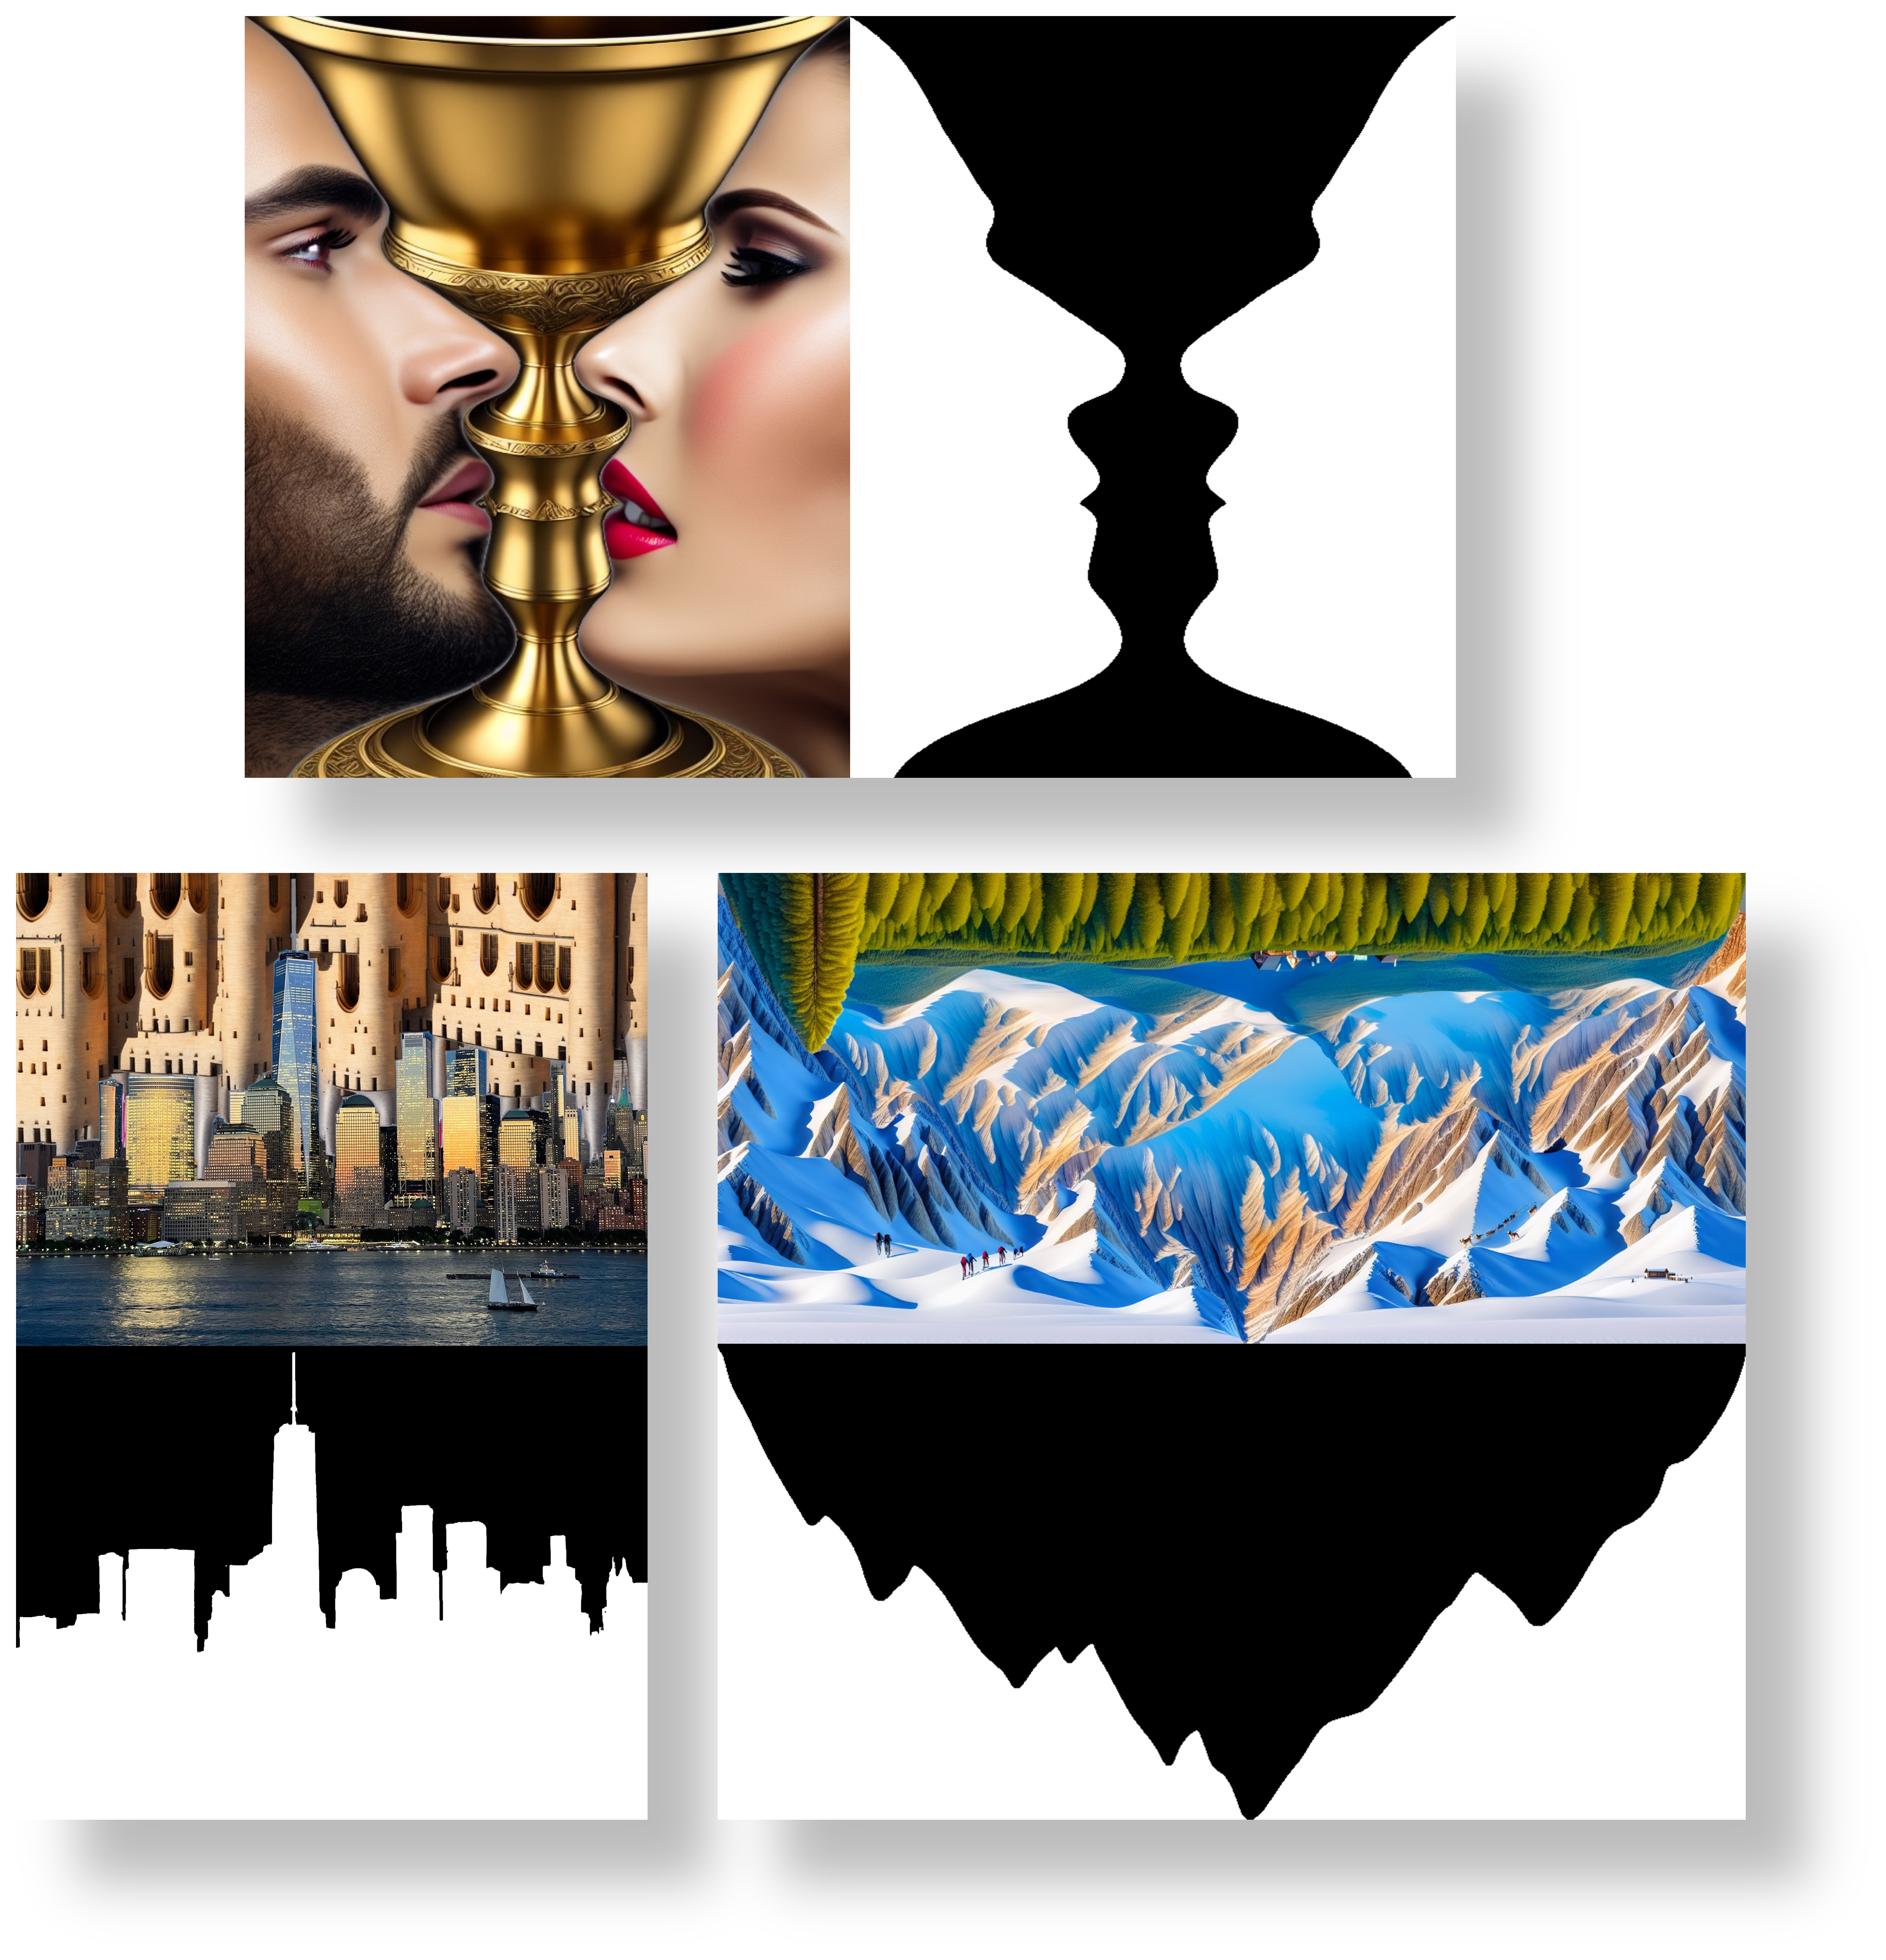
\includegraphics[width=1\linewidth]{figs/illusions.pdf} % For some reason I can't explain, this figure crashes PDF readers on my iPhone - but not on my laptop. No idea why. But I'll replace it with a png.
    \includegraphics[width=1\linewidth]{figs/NonCrashyIllusions.png}
    \hspace{-40pt}
    \caption{\textbf{Optical Illusions}: Our Alpha-to-RGB algorithm from \cref{sec:application_alpha_to_rgb} can be used to generate striking optical illusions. In each image, we use two prompts: one for each region of the alpha mask. On the top image, we fill in the classic goblet illusion: we use the prompts ``man and woman staring at each other'' along with ``a brass goblet''. On the bottom right image, we use the prompts ``a mountain range with snow-capped mountains'' and ``a mountain range with snow-capped mountains behind a dense green forest''. The log cabins and skiers were added after the fact for decoration. And on the left, a photograph of new york city was cut out, and the remaining mask was given the prompt ``a medieval castle'' and flipped upside-down and composited back onto the image of the city. Please view them upside-down! }
    \label{fig:illusions}
\end{figure*}


\begin{figure*}
    \centering
    % \includegraphics[width=1\linewidth]{figs/magick_styles_a.jpg}
    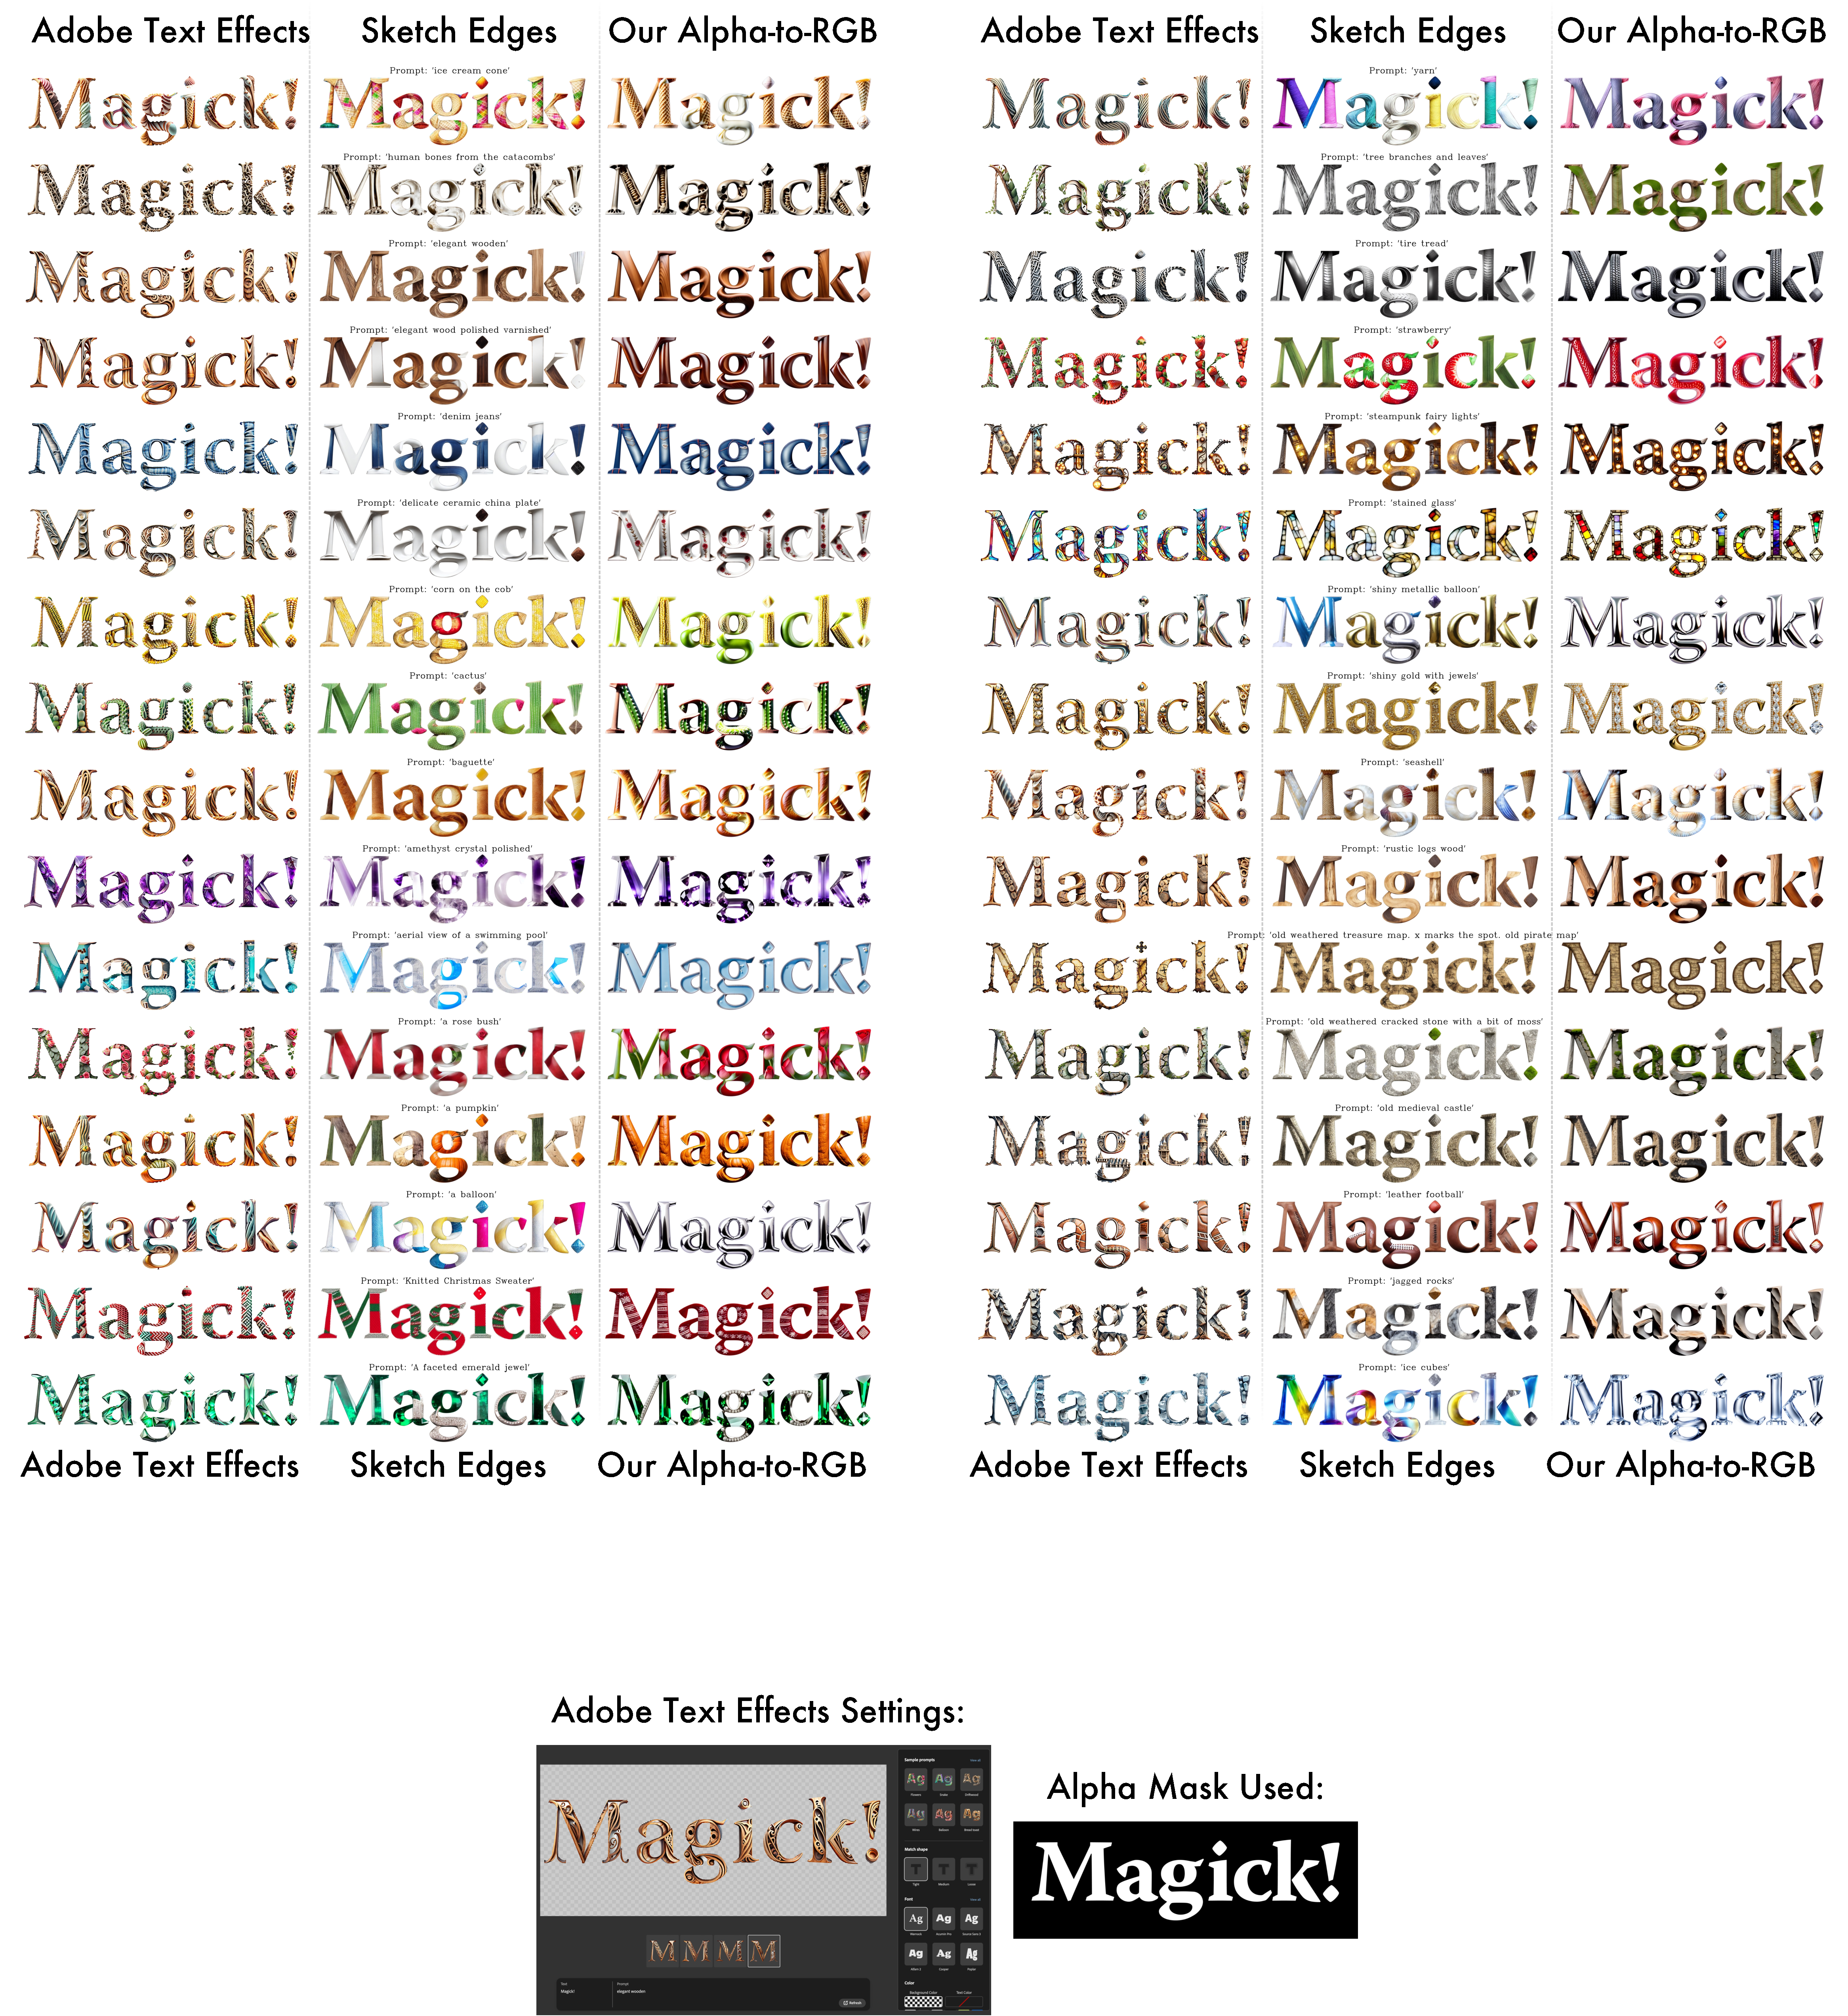
\includegraphics[width=1\linewidth]{figs/verymagick.pdf}
    \caption{\textbf{Text Stylization:} \textit{This image is very high resolution - please zoom in!} We apply our Alpha-to-RGB algorithm from \cref{sec:application_alpha_to_rgb} to the text ``Magick!'' in the font ``Warnock'', using many different styles. We compare it to two baselines: Adobe Text Effects and our Sketch Edges baseline from \cref{sec:application_alpha_to_rgb}. Note how the results from Adobe Text Effects don't always conform to the text boundary properly, despite the settings given to it (also depicted in this figure - its boundary mode is set to ``tight''). We chose to include the Sketch Edges baseline instead of the Canny Edges baseline because in our user study \cref{fig:user_results} it was the stronger-preferred of the two baselines.}
    \label{fig:magick_styles}
\end{figure*}


\begin{figure*}
    \centering
    \includegraphics[width=.7\linewidth]{figs/chess_swirl.jpg}
    \caption{Some more results of our Alpha-to-RGB algorithm \ref{sec:application_alpha_to_rgb}. The alpha masks are inverted for visibility.}
    \label{fig:swirly_chess}
\end{figure*}


\begin{figure*}
    \centering
    \includegraphics[width=1\linewidth]{ddpack0_q90.jpg}
    \caption{\textbf{Dataset Samples Part 1/4}: \textbf{Text Stylization:} \textit{This image is very high resolution - please zoom in!} This figure displays 325 random samples from our dataset, along with their alpha masks. Each sample also has a caption, not shown here.}
    \label{fig:dataset1of4}
\end{figure*}


\begin{figure*}
    \centering
    \includegraphics[width=1\linewidth]{figs/ddpack1_q90.jpg}
    \caption{\textbf{Dataset Samples Part 2/4}: \textbf{Text Stylization:} \textit{This image is very high resolution - please zoom in!} This figure displays 325 random samples from our dataset, along with their alpha masks. Each sample also has a caption, not shown here.}
    \label{fig:dataset2of4}
\end{figure*}

\begin{figure*}
    \centering
    \includegraphics[width=1\linewidth]{figs/ddpack2_q90.jpg}
    \caption{\textbf{Dataset Samples Part 3/4}: \textbf{Text Stylization:} \textit{This image is very high resolution - please zoom in!} This figure displays 325 random samples from our dataset, along with their alpha masks. Each sample also has a caption, not shown here.}
    \label{fig:dataset3of4}
\end{figure*}

\begin{figure*}
    \centering
    \includegraphics[width=1\linewidth]{figs/ddpack3_q90.jpg}
    \caption{\textbf{Dataset Samples Part 4/4}: \textbf{Text Stylization:} \textit{This image is very high resolution - please zoom in!} This figure displays 325 random samples from our dataset, along with their alpha masks. Each sample also has a caption, not shown here.}
    \label{fig:dataset4of4}
\end{figure*}


%%%%%%%%% REFERENCES


% \end{document}
